\section{Termocoppie e termopile}
Per far si che si possa generare della corrente elettrica le
termocoppie sono costituite da due circuiti metallici di materiale
differente ($M_1$, $M_2$) saldati assieme nei punti dove si
campiona la temperatura di riferimento $T_1$ e la temperatura
da misurare $T_2$.

\begin{figure}[htbp]
	\centering
	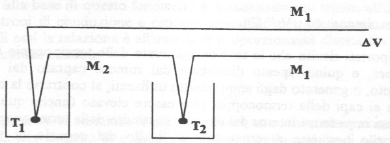
\includegraphics[scale=0.5]
			{img/termocoppia.png}
	\caption{Termocoppia\label{fig:termocoppia}}
\end{figure}

A questo punto se le temperature dove ci sono le saldature sono
differenti si genera della differenza di potenziale $\Delta V$ che
cresce all'aumentare della differenza $T_2-T_1$.
In questo modo possiamo creare una relazione di tipo lineare per
descrivere l'andamento della tensione rispetto alla variazione di
temperatura, invece useremo una relazione non lineare quando la
differenza termica è di qualche decina di °C:

	\[\Delta V = a(T_2 -T_1)\]
	\[\Delta V = a(T_2-T_1)+b(T_2-T_1)^2+c(T_2-T_1)^3+ ...\]

dove i valori di $a$, $b$, $c$ dipendono dai materiali utilizzati.

Un problema delle termocoppie è che la tensione fornita è piccola e
quindi più sensibile al rumore, per questo vengono usate le termopile,
cioè più termocoppie collegate in serie.

\begin{figure}[htbp]
	\centering
	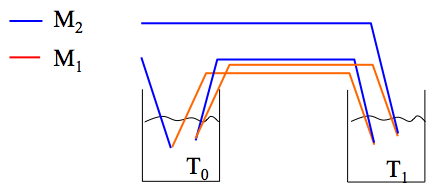
\includegraphics[scale=0.5]
			{img/termopila.png}
	\caption{Termopila\label{fig:termopila}}
\end{figure}

Indicando con $n$ il numero di termocoppie collegate in serie, la
tensione misurata sulla termopila sarà:

	\[\Delta V = na(T_2 -T_1)\]

\section{Termo-resistenze}
Sono resistenze il cui valore cresce con  la temperatura e vengono
spesso indicate dalla  sigl a PTC (Positive Temperature
Coefficient). La relazione  che lega la temperatura assoluta al
valore della resistenza è la seguente:

	\[R=kT_{ass}\]

Volendo però fornire un'approssimazione più realistica introduciamo un
coefficiente alfa, detto coefficiente di temperatura:

	\[\alpha=\frac{1}{R_0}[\frac{dR}{dT}]\]

con R0 e T0 valori di riferimento.

\section{Termistori}
Come le termo-resistenze variano la loro resistività in funzione
della temperatura; sono spesso indicati con la sigla o  NTC (Negative
Temperature Coefficient). La relazione fra la resistività e la
temperatura è la seguente:

	\[R=R_0e^{-D(\frac{1}{T_0}-\frac{1}{T})}\]

dove $R_0$ indica la resistenza di riferimento ad una data
temperatura $T_0$; $B$ è la costante di temperatura

I termistori sono preferibili alle termo-resistenze quando le
variazioni di temperature sono limitate.

\section{Trasduttori integrati di temperatura}
si tratta di circuiti integrati comprendenti una giunzione a
semiconduttore, la cui caratteristica tensione-corrente dipende
fortemente dalla temperatura. La soluzione circuitale più semplice è
rappresentata da due diodi identici alimentati da correnti differenti

\begin{figure}[htbp]
	\centering
	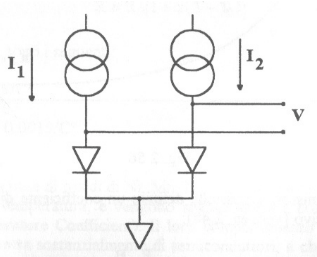
\includegraphics[scale=0.5]
			{img/termointegrati.png}
	\caption{Trasduttori integrati di temperatura
\label{fig:termointegrati}}
\end{figure}


Fissata la corrente entro la giunzione, la caduta di tensione viene
utilizzata come misura della temperatura ed opportunamente
amplificata:

	\[V=\frac{KT}{e}\ln(\frac{I_2}{I_1})\]

questo vale, se e sole se vale la seguente relazione per ogni diodo:

	\[V_d=\frac{KT}{e}\ln(\frac{I_d}{I_0})\]